\part{Analysis}  \label{part:analysis}

\chapter{Methodology}

In this chapter, we will present the methodology used to analyze our solution. Our tests were focused on the data retrieval as we considered it to be the part that needed to be evaluated the most. This is mainly due to the fact that our solution will be considered viable only if it do not stress intensively the network. Because we are talking about Internet of Things, and particularly Wireless Sensors Network, preserving the battery life of nodes is a must. This can be done by maximizing the CPU sleep time, or reducing the transmission or reception time. For those particular reasons, five criteria designed our tests:

\begin{itemize}
  \item CPU duty time
  \item CPU low power mode time
  \item Radio transmission time (Tx)
  \item Radio reception time(Rx)
  \item Amount of packets induced by our solution \\
\end{itemize}

The four first arguments can give an estimate of the energy consumption. With that we can build a model to tell whether if our solution depletes the battery too much. Dunkel et al. \cite{dunkels2007software} demonstrate that energy consumption can be given by the following formula

\begin{equation}
  E = (I_m t_m + I_l t_l + I_t t_t + I_r t_r) * V
\end{equation}

where $I_m$ and $t_m$ represents the current draw of the microprocessor when running and the time in which it has been running respectively. $I_l$ and $t_l$  are the current draw and the time of the microprocessor in low power mode. $I_t$ and $t_t$ are the current draw and the time of the communication device in transmit mode while $I_r$ and $t_r$ are the current draw and the time of the communication device in receive mode. Finally, $V$ is the supply voltage. The $I_m$, $I_l$, $I_t$, $I_r$ and $V$ values are device dependent. Different models can present different values. The Tab.\ref{table:device_consumption} shows such values for different models.\\

\begin{table}
  \centering

  \begin{tabular}{|c|c|c|c|c|c|}
    \hline
    Model & $I_m$ (mA) & $I_l$ (mA) & $I_t$ (mA) & $I_r$ (mA) & $V$ (V)\\
    \hline
    Zolertia Z1 & 5 & 0.0005 & 17.4 & 18.8 & 3 \\
    \hline
    Tmote Sky & 1.8 & 0.0545 & 19.5 & 21.8 & 3 \\
    \hline
  \end{tabular}
  \caption{Devices electrical characteristics}
  \label{table:device_consumption}
\end{table}

To implement our benchmarks, we used the couple Contiki-OS and Cooja. The former was used to configure the nodes while the latter was used to simulate those nodes. For more details on those two, see Chap.\ref{chap:contiki}.\\

This chapter will be organized in two sections. First, we will explain the different configurations (number and role of nodes) used for our benchmarks. Secondly, we will explain in more detail the mechanisms used for nodes to send their data. The code used to implement those parts can be found on our public repository \textit{\href{https://github.com/edd19/netflow_contiki}{netflow\_contiki}} on github.

\section{Configurations}
\todo[inline]{explain packet rate}
Four different configurations were used for the purpose of our tests. They all differ by the facts that nodes send IPFIX messages or TinyIPFIX messages  or simply none. However they all share the common components of WSN: sensor nodes and gateway node.

\begin{description}
  \item[Simple] In this configuration, the nodes do not send information about the flows they observed or any meta information about their network. They only occupy the role of sensor nodes, meaning sensing the environment and transmitting the values observed.
  \item[Ipfix] This configuration is an upgrade of the previous one where the nodes now send informations about the flows they observerd. Those informations are formatted using the full IPFIX format. The gateway node do not need to do any conversion and the data is hence transmitted directly to the collector.
  \item[TinyIpfix] This configuration is also an upgrade of the \textit{Simple} configuration. The nodes send flows informations but using the TinyIPFIX format. This imply that the gateway node do conversion of TinyIPFIX to IPFIX before transmitting the data to the collector.
  \item[Aggregation] This last configuration adds aggregators to the \textit{TinyIpfix} configuration. Aggreagators collect TinyIPFIX messages and merge them in one message. They then send those merged messages to the gateway who will convert them to compliant IPFIX messages. In return the gateway node will send the converted messages directly to the collector. \\
\end{description}

The Tab.\ref{table:configurations} resumes the different configurations used during our benchmarks. \\

\begin{table}
  \centering
  \begin{tabular}{|c|c|c|}
    \hline
    Configuration & Monitoring deployed & Aggregator \\
    \hline
    Simple & None & No \\
    \hline
    Ipfix & IPFIX & No \\
    \hline
    TinyIpfix & TinyIPFIX & No \\
    \hline
    Aggregation & TinyIPFIX & Yes \\
    \hline
  \end{tabular}
  \caption{Configurations used}
  \label{table:configurations}
\end{table}

We tested each configuration with an increasing number of nodes of 5, 10, 15 and 20. Each configuration was tested for 25 minutes. The number of nodes was limited by the computer used during benchmarking as it proved unable to simulate more than 20 nodes with Cooja. We also tested the influence of the sending time of the IPFIX messages with a 1 and 5 minutes interval between each message.\\

Also for each simulation we keep track of the following informations:
\begin{itemize}
  \item The 4-uple (Rx, Tx, Cpu, Lpm) where Rx is the radio reception time, Tx the radio transmission time, Cpu the time the Cpu is working and Lpm the time the Cpu is sleeping. This 4-uple was recorded for each minute. This gave an idea on how the energy consumption evolves minute by minute.
  \item A log of all the packets sent during the simulation thanks to a Cooja plug-in. This permits to have an idea on the amount of traffic generated by our solution.\\
\end{itemize}

Our tests were done solely on simulation using the Cooja simulation software. The nodes used during the simulations were the Zolertia Z1. Also we considered a setup for all configurations were the radio loss was null. Also all motes were fixed meaning they did not move during the simulation.

\section{Sending of data}

This section will answer the questions relative on how the motes send IPFIX/TinyIPFIX messages, what triggers the sending of those meta informations and what particular informations are sent. Distinction must be done on the three types of motes: exporter, aggregator and gateway.\\

\begin{description}
  \item[Exporter] It is straighforward. It first send the templates then set a timer. When the timer expired or when the flows table reached its maximum capacity, the exporter exports the records. All packets, templates or data, are sent whether directly to the gateway or to an aggregator node depending on the configuration. The Alg.\ref{algo:exporter} is the algorithm corresponding to an exporter.

  \begin{algorithm}
    \textbf{Function} Exporter:\\
    send templates\;
    set timer\;
    \While{true}{
      yield process until event\;
      \If{timer timeout or flows table is full}{
        send data/records\;
        empty flows table\;
        reset timer\;
      }
    }
   \caption{Exporter algorithm}
   \label{algo:exporter}
  \end{algorithm}

  \item[Aggregator] It is an extension of the Exporter. It both merge and send TinyIPFIX messages. At first it send the templates used then also set a timer. When the aggregator received an TinyIPFIX message, it merged that one with previous ones if any. When a timeout of the timer occured or when the flows table of the aggregator reached its limit, it will merge its records with the ones received then will send the new formed message to the gateway. This behavior is shown by the Alg.\ref{algo:aggregator}.

  \begin{algorithm}
    \textbf{Function} Aggregator:\\
    send templates\;
    set timer\;
    \While{true}{
      yield process until event\;
      \If{received TinyIPFIX message}{
        merge message with previous ones\;
      }
      \If{timer timeout or flows table is full}{
        merge aggregator data/records with received ones\;
        send merged messages\;
        empty flows table\;
        reset timer\;
      }
    }
   \caption{Aggregator algorithm}
   \label{algo:aggregator}
  \end{algorithm}

  \item[Gateway] It convert TinyIPFIX messages received into IPFIX message. The converted messages are sent directly to the collector. This is shown by Alg.\ref{algo:gateway}.

  \begin{algorithm}
    \textbf{Function} Gateway:\\
    \While{true}{
      yield process until event\;
      \If{received TinyIPFIX message}{
        convert into IPFIX message;
        send converted message;
      }
    }
   \caption{Gateway algorithm}
   \label{algo:gateway}
  \end{algorithm}

\end{description}

Two templates were used during our tests. The first template (Tab.\ref{table:traffic_template}) was used to send traffic information about the network while the second one (Tab.\ref{table:meta_info_template}) to obtain meta-information about nodes. The first template considers records of size of 8 bytes. Each record contains the source node id, the destination node id which is the receiving end of a flow and also the number of octets for that particular flows plus the number of packets. This template is the most often used. The second template with records of size of 5 bytes is comprised of the source node id but also the parent node id (in RPL routing) and also the remaining battery of the node. This template is not sent often. It must be sent on update of the parent or at interval of one hour. The fields source node id, destination node id, parent node id and battery were defined for the purpose of this thesis. They are not standard ones.

\begin{table}
  \centering
  \begin{tabular}{|c|c|}
    \hline
    Source Node Id & 2 bytes \\
    \hline
    Destination Node Id & 2 bytes \\
    \hline
    Octets delta count & 2 bytes \\
    \hline
    Packets delta count & 2 bytes \\
    \hline
  \end{tabular}
  \caption{Traffic template}
  \label{table:traffic_template}
\end{table}

\begin{table}
  \centering
  \begin{tabular}{|c|c|}
    \hline
    Source Node Id & 2 bytes \\
    \hline
    Parent node id & 2 bytes \\
    \hline
    Battery & 1 byte \\
    \hline
  \end{tabular}
  \caption{Meta-information template}
  \label{table:meta_info_template}
\end{table}

\chapter{Results}

After having presented our methodology used when testing our solution, this chapter will present and discuss the results obtained from it.

\section*{Energy consumption}

The Fig.\ref{fig:average_energy} shows the average energy consumption in term of mJ by minute for the nodes. The bar charts shows the evolution of the energy consumption with increasing number of nodes (5, 10, 15 and 20) for the three configurations \textit{simple}, \textit{tipfix} and \textit{aggrega}. As a reminder, the \textit{simple} configuration has no monitoring done with TinyIPFIX while the two has monitoring activated by the mean of TinyIPFIX messages. The different between \textit{tipfix} and \textit{aggrega} configurations lies in the fact that the \textit{aggrega} has aggregator nodes that merge TinyIPFIX messages into one. \\

\begin{figure}[h]
  \centering
  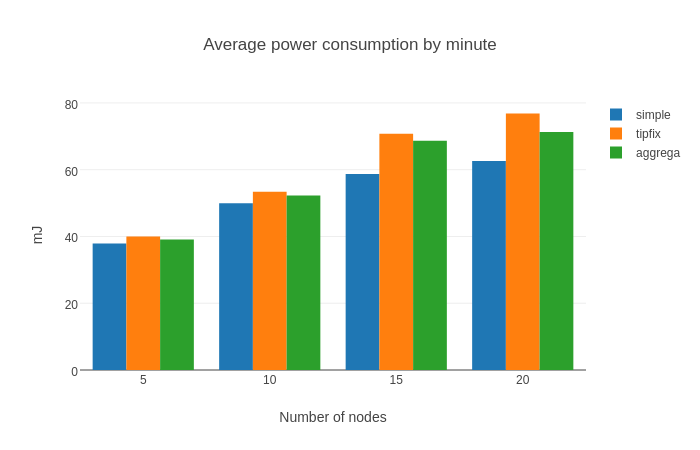
\includegraphics[width=\textwidth]{res/average_energy.png}
  \caption{Average energy consumption in mJ by minute}
  \label{fig:average_energy}
\end{figure}

From the chart we can conclude that by using aggregators inside the network we can reduce the added energy consumption induced by the usage of TinyIPFIX messages for monitoring purposes. As can be clearly seen when introducing more nodes, the energy consumption increases much more when not using aggregators. The graph on Fig.\ref{fig:increase_energy} shows exactly how the monitoring increase the energy consumption. The increase was computed by comparing the simple and aggrega configurations on their counterpart the simple configuration which do not send any information about the status of the network. As one may notice, the tipfix configuration consumes  relatively more energy when the number of nodes increases. However, it appears not to be the case with the aggrega one. Reasons may be due to the positions of the aggregators who impact greatly how the network behaves and thus weight on the power consumption. By placing intelligently the aggregators it is therefore possible to stress less the network.\\

\begin{figure}[h]
  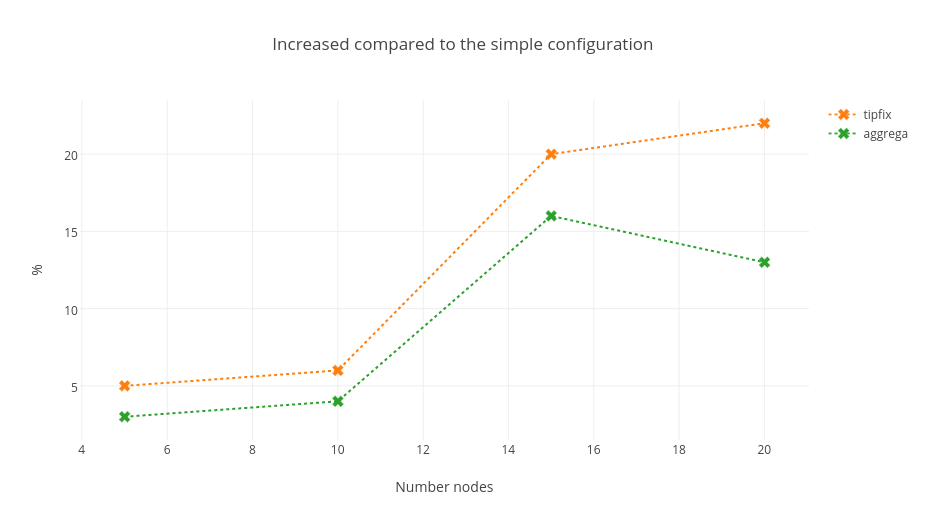
\includegraphics[width=\textwidth]{res/increase_energy.png}
  \caption{Increase in energy consumption induced by monitoring}
  \label{fig:increase_energy}
\end{figure}

\todo[inline]{explain why for 5 nodes exporters consume more}
One of the big advantage of also using aggregators is that it reduced drastically the load on the nodes that simply exports data and do not merge messages. This is depicted in Fig.\ref{fig:aggrega_energy}. The bar chart represents the energy consumption for the exporters and the aggregators in the aggrega configuration. Apart from the case with 5 number of nodes, all the case shows clearly that the exporters consume less energy than the aggregators with almost 20 mJ of difference for 15 nodes.\\

\begin{figure}[h]
  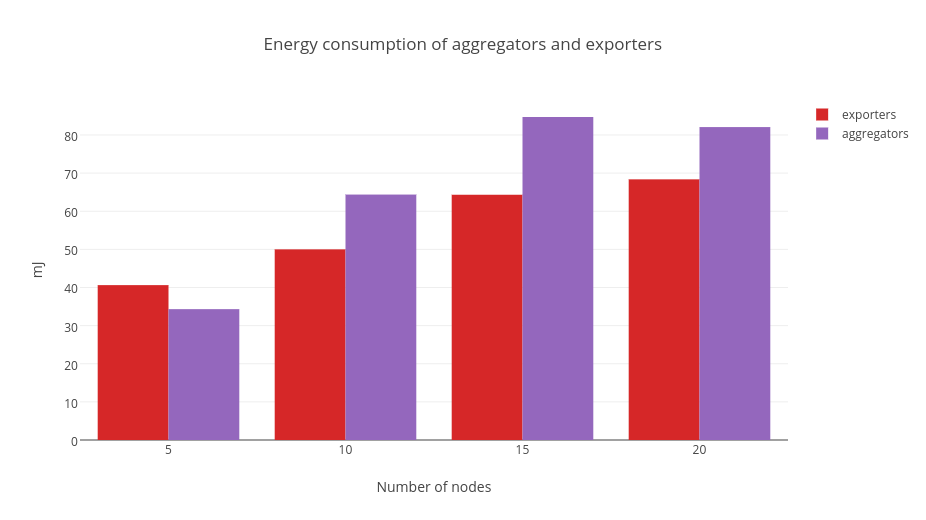
\includegraphics[width=\textwidth]{res/energy_aggrega}
  \caption{Energy consumption between aggregators and exporters}
  \label{fig:aggrega_energy}
\end{figure}

With those results, one may wonder how it affects the battery life of the nodes. The estimated lifetime of the battery is indicated in Tab.\ref{tab:battery_lifetime}. To compute those estimations we used the following formula

\begin{equation}
  lifetime = \frac{2400 mAh * 2}{X mW * 24 hours}
\end{equation}

where $X$ is the power consumption of a node. We used $2400mAh$ as we considered that the nodes were powered by AA battery. We multiply it by $2$ as the \textit{Zolertia Z1} uses 2 batteries. \\

The table shows clearly that to preserve the battery lifetime, aggregators become a must the more nodes are present in the IoT network.

\begin{table}
  \centering
  \begin{tabular}{|c|c|c|c|c|}
    \hline
    configuration & 5 nodes & 10 nodes & 15 nodes & 20 nodes \\
    \hline
    simple & 317 days & 240 days & 204 days & 190 days\\
    \hline
    tipfix & 300 days & 224 days & 168 days & 156 days\\
    \hline
    aggrega (exporters) & 294 days & 240 days & 186 days & 174 days \\
    \hline
  \end{tabular}
  \caption{Battery lifetime for different configurations}
  \label{tab:battery_lifetime}
\end{table}

\section*{Nodes usage time}

So as to more understand the power consumption induced by our solution, there is a need to see how often the nodes are active, and when it is the case what are they doing. To do so, we kept track on the time the nodes spend with their microprocessor active or in low power mode but also the time they were transmitting or receiving data via radio. This is what Fig.\ref{fig:time_all} shows. The Fig.\ref{fig:cpu_time} shows the average time the microprocessor is active by minute while Fig.\ref{fig:lpm_time} shows the average time the microprocessor is in low power mode. Fig.\ref{fig:tx_time} and Fig.\ref{fig:rx_time} shows average transmission time and receiving time by minute for a node. \\

\begin{figure}[h]
    \centering
    \begin{subfigure}[b]{0.45\textwidth}
        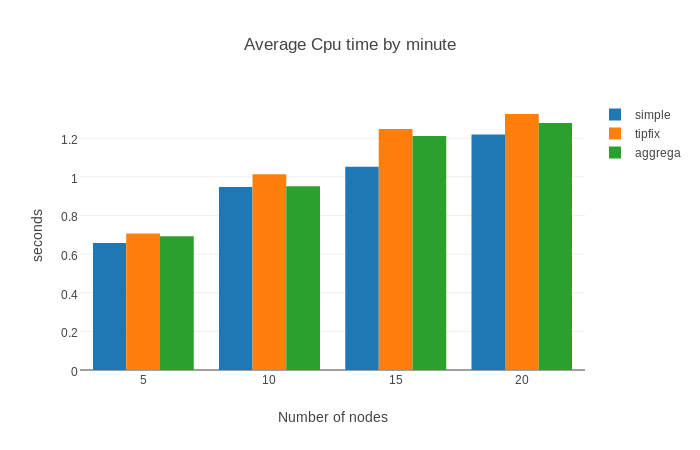
\includegraphics[width=\textwidth]{res/average_cpu}
        \caption{Average time spent with CPU active}
        \label{fig:cpu_time}
    \end{subfigure}
    ~
    \begin{subfigure}[b]{0.45\textwidth}
        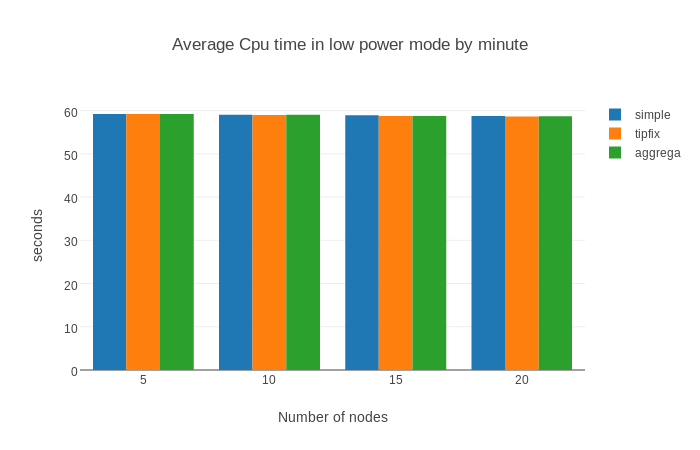
\includegraphics[width=\textwidth]{res/average_lpm}
        \caption{Average time spent with CPU in low power mode}
        \label{fig:lpm_time}
    \end{subfigure}
    ~
    \begin{subfigure}[b]{0.45\textwidth}
        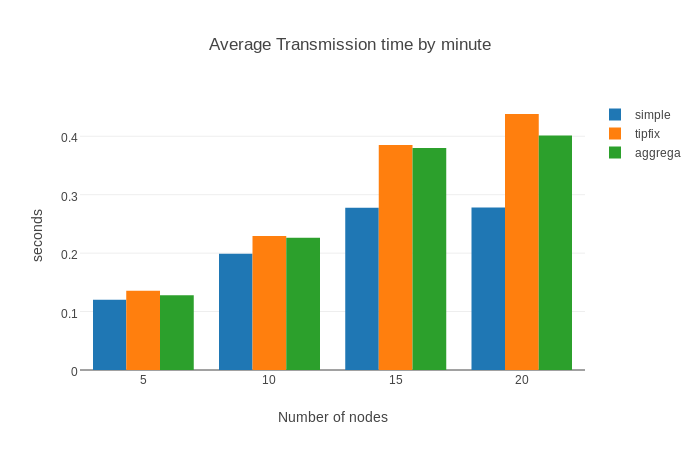
\includegraphics[width=\textwidth]{res/average_tx}
        \caption{Average time spent in transmission mode}
        \label{fig:tx_time}
    \end{subfigure}
    ~
    \begin{subfigure}[b]{0.45\textwidth}
        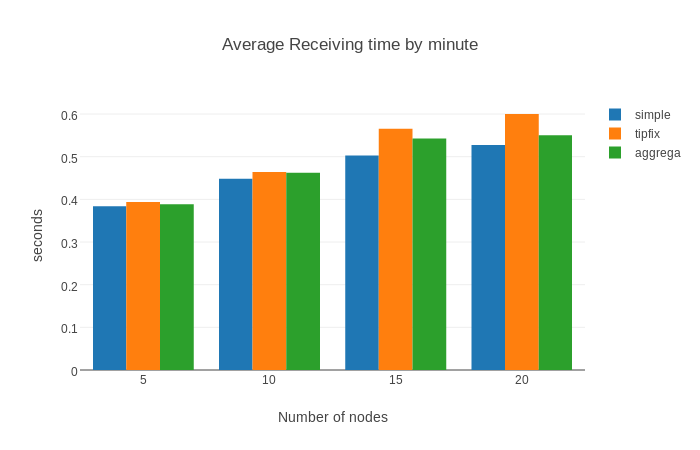
\includegraphics[width=\textwidth]{res/average_rx}
        \caption{Average time spent in receiving mode}
        \label{fig:rx_time}
    \end{subfigure}
    \caption{Average components time of nodes}
    \label{fig:time_all}
\end{figure}

The differences between the three configurations is highly visible for the transmission time and receiving time. In Fig.\ref{fig:tx_time} who shows the transmission time, we can clearly see than by monitoring, nodes pass more time transmitting data which influence the receiving time of the nodes. On Fig.\ref{fig:rx_time}, who shows receiving time, we can see that nodes receive more data which needs to be routed. It is however in the transmission time than there is the most gap between the configurations without and with TinyIPFIX.
